\section{Exercise 2: PDN impedance in the frequency domain}

%%%%%%%%%%%%%%%%%%%%%%%%%%%%%%%%%%%%%%%%%%%%%%%%%%%%%%%%%%%

\subsection{AC analysis of the PDN}

To compute the impedance of the PDN seen from the die interface, a very simple netlist, \texttt{pdn\_ac.cir}, has been written. It includes the
complete netlist \texttt{pdn.cir} created in the previous exercise, so that the PDN is exactly the same one (without decoupling capacitors), and it
adds only the excitation and the analysis directive.

\noindent\\ The impedance is obtained with a \textit{test current}: an AC current source of $1\,\text{A}$ is connected to the node \texttt{vdie}, which
is the die interface (the port where the impedance is requested).\\ By definition, the impedance seen from a port is the ratio between the voltage across
the port and the current entering it:
\begin{equation}
  Z(f) = \frac{V(f)}{I(f)}\,
\end{equation}
\noindent\\ Since the injected current has a magnitude of $1\,\text{A}$, the voltage at \texttt{vdie} is numerically equal to the impedance:
$Z(f) = V(\texttt{vdie})/1\,\text{A}$. The other sources do not affect the result: in an AC analysis the ideal $1\,\text{V}$ source of the VRM behaves
as a short circuit, and the PWL current load of the die has no AC magnitude, so it does not contribute. The only excitation is therefore the test
current, and the analysis describes the passive network alone.

\noindent\\ The AC analysis is performed from $1\,\text{Hz}$ to $5\,\text{GHz}$, with a logarithmic sweep of 1000 points per decade. The corresponding
part of the netlist is shown in \autoref{lst:pdn_ac}, while the plot of $|Z|$ obtained with LTspice is shown in \autoref{fig:zdie_nodecaps}.

\begin{lstlisting}[language=ltspice, caption={Netlist \texttt{pdn\_ac.cir} used for the AC analysis.}, label={lst:pdn_ac}]
.include "../eser1/pdn.cir"

* AC test current into the die node (the "Port1" of the slide schematic)
Iac 0 vdie DC 0 AC 1
.ac dec 1000 1 5G
.meas ac zmax MAX mag(V(vdie))
.meas ac fpk  WHEN mag(V(vdie))=zmax
.meas ac z100M FIND mag(V(vdie)) at 100Meg
.end
\end{lstlisting}

\begin{figure}[!h]
\centering
% Replace the placeholder below with the LTspice plot:
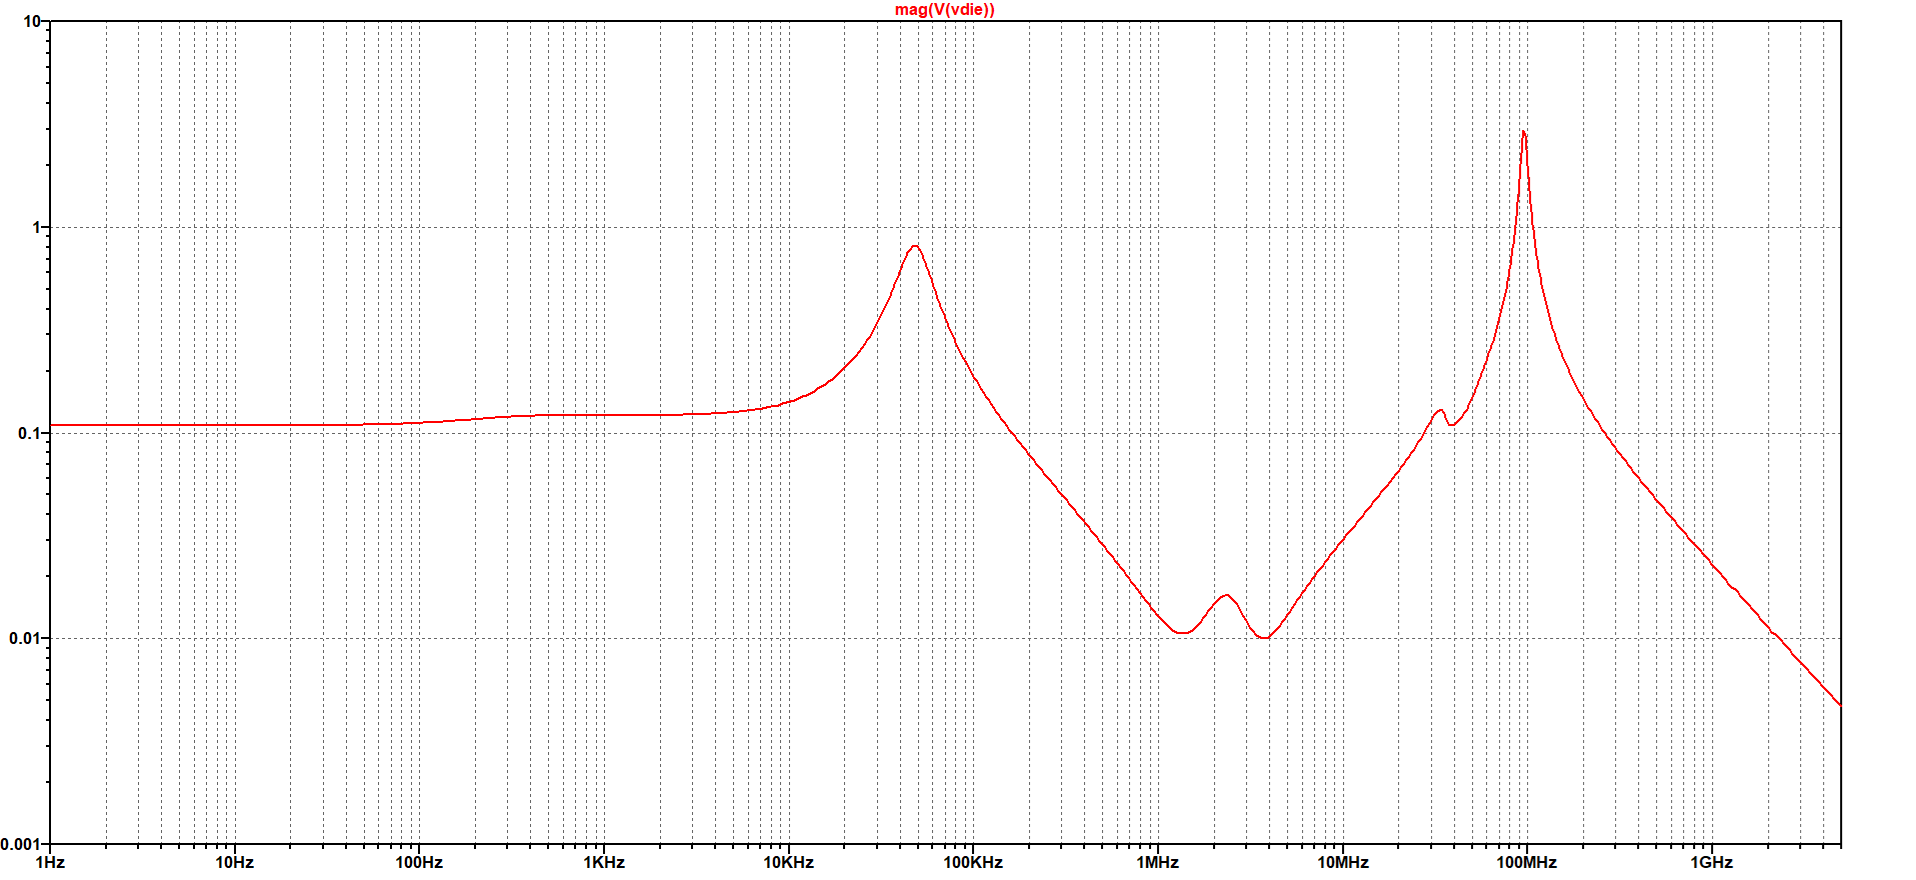
\includegraphics[width=0.95\textwidth]{./eser2/pdn_ac.png}
%\fbox{\parbox{0.9\textwidth}{\centering\vspace{3cm} Figure placeholder: LTspice plot of $|Z|$ at the die port, without decoupling capacitors\vspace{3cm}}}
\caption{Impedance magnitude seen from the die interface (node \texttt{vdie}) of the PDN without decoupling capacitors, from $1\,\text{Hz}$ to $5\,\text{GHz}$.}
\label{fig:zdie_nodecaps}
\end{figure}

\noindent From the Figure reported above, it is possible to see that the impedance
reaches the peak value of $|Z|_{\max} \approx 3~\Omega$ at the frequency $f_{\text{peak}} = 96~\text{MHz}$,
in line with the expected behaviour of the PDN. Moreover, exploiting the \texttt{.meas} statements in the netlist,
LTspice automatically computes the peak value and the corresponding frequency, which are reported in the log file \texttt{pdn\_ac.log}.
\\ The values reported in the log file are:
\[
|Z|_{\max} = 3.057~\Omega, \quad f_{\text{peak}} = 95.94~\text{MHz}
\]

%%%%%%%%%%%%%%%%%%%%%%%%%%%%%%%%%%%%%%%%%%%%%%%%%%%%%%%%%%%
\newpage
\subsection{Choice of the frequency range}

The upper limit of the sweep, $5\,\text{GHz}$, is set by the bandwidth of the models. The board and the package macromodels have been obtained
from S-parameter data, \texttt{board.ts} for the board and \texttt{package\_ports\_on\_caps.ts} for the package, that cover a limited frequency range,
and a rational macromodel is reliable only inside the range of the data it was fitted to. In particular:
\begin{itemize}
  \item the board model has been fitted over a bandwidth of $5\,\text{GHz}$ (as stated in the header of \texttt{board\_passive.cir});
  \item the package model has been fitted over a bandwidth of $10\,\text{GHz}$ (as stated in the header of the package macromodel file);
  \item the die model is a lumped RC network, and it has no frequency limit of its own.
\end{itemize}
The validity of the whole PDN is therefore limited by the narrowest model, the board, and this is why the analysis stops at $5\,\text{GHz}$. Above
this frequency the simulator still returns numbers, but they are only an extrapolation of the models, and they would not be a trustworthy
description of the real network. Moreover, the reference curve shown in the assignment also stops at about $5\,\text{GHz}$.

\noindent\\ The lower limit of $1\,\text{Hz}$ has been chosen to include the whole behaviour of the network, down to the region where the impedance
no longer changes: at the lowest frequencies it is flat and equal to the DC resistance of the PDN. The S-parameter data start from DC, so the models
are valid there, and extending the sweep downwards has a negligible cost, since the whole analysis takes less than a second.